\documentclass[UTF8,11pt,a4paper]{ctexart}
\usepackage[margin=2.15cm]{geometry}
\usepackage{amsmath,amssymb,bm,booktabs,longtable,array,graphicx,xcolor,hyperref,float,caption}
\hypersetup{colorlinks=true,linkcolor=blue!55!black,urlcolor=blue!55!black}
\graphicspath{{../../}}
\setlength{\parindent}{2em}
\setlength{\parskip}{0.35em}
\definecolor{good}{RGB}{26,120,74}
\definecolor{warn}{RGB}{180,92,20}
\definecolor{deep}{RGB}{30,58,95}
\newcommand{\mat}[1]{\bm{#1}}
\newcommand{\code}[1]{\texttt{#1}}
\newcommand{\key}[1]{\textcolor{deep}{\textbf{#1}}}

\title{\textbf{高频变压器匝级 GNN：网络、数据、指标与在线参数辨识作用}\
\large EXP16--EXP18 项目学习与掌控说明书}
\author{基于当前仓库代码与已保存实验结果整理}
\date{2026年9月10日}

\begin{document}
\maketitle
\begin{abstract}
本文档回答五个问题：当前网络究竟输入什么、内部怎样计算、输出什么；训练“真值”怎样由物理矩阵模型产生；图和指标分别表达什么；现有精度能证明什么、不能证明什么；以及这些工作如何服务最终的在线参数辨识。最重要的结论是：\key{EXP18 当前是匝级图的正向代理模型，而不是从实测波形直接反演内部参数的最终在线辨识器}。它验证了图表示、物理教师和多任务输出链可行，并暴露了参数非唯一性、无源性和局部定位三个关键难点。EXP17 的 Fisher/OED 结果则说明，未来在线阶段不能自由辨识全部矩阵元素，而应只更新可观测的低维图参数子空间。
\end{abstract}
\tableofcontents
\newpage

\section{先用一张路线图理解整个工程}

当前工程可分为三层：
\begin{center}
\fbox{\parbox{0.91\linewidth}{
\centering
\textbf{物理教师层（已实现）}：匝级 $\mat R,\mat L,\mat C$ 与精确矩阵/Kron 求解器\\
$\Downarrow$ 生成端口导纳、内部节点电压、跨绕组位移电流真值\\[0.3em]
\textbf{GNN 正向代理层（EXP16/18，已实现）}：匝级异构图 $+$ DAB 工况 $\rightarrow$ 快速预测上述响应\\
$\Downarrow$ 为以后反演提供可微、快速、保留内部结构的前向模型\\[0.3em]
\textbf{在线反演层（尚未实现）}：实测 $v_1,i_1,v_2,i_2$ $\rightarrow$ 低维图参数修正 $\rightarrow$ 物理解码与响应重构
}}
\end{center}

因此，现阶段回答的是“\emph{给定一个匝级参数图，GNN 能否快速复现它的外部和内部响应？}”；最终目标才是“\emph{给定真实运行波形，哪些内部参数变化能够被稳定反推？}”。这一区分是理解所有结果的钥匙。

\section{物理对象：从梯形网络到矩阵方程}

\subsection{为什么一匝作为一个节点}

原、副边分别有 $N_p,N_s$ 匝，总节点数 $N=N_p+N_s$。当前路线不再研究如何把若干匝合成一段，而是直接采用“一匝一节点”。节点保存该匝的归属、位置、端口身份和局部参数；边表示导电连接、电容耦合或磁耦合。这样既保留传统梯形网络的纵向连接，又允许非相邻匝之间存在远程耦合。

\subsection{核心矩阵方程}

支路电流与节点电压的频域关系写成
\begin{equation}
 \mat Y_n(j\omega)=
 \mat A(\mat R+j\omega\mat L)^{-1}\mat A^{\mathsf T}
 +\mat G+j\omega\mat C,
 \label{eq:yn}
\end{equation}
其中 $\mat A$ 是支路--节点关联矩阵，$\mat R$ 为电阻矩阵，$\mat L$ 包含自感和互感，$\mat C$ 为 Maxwell/网络电容矩阵，$\mat G$ 表示介质或对地损耗。将节点分成外部端口 $p$ 与内部节点 $i$：
\begin{equation}
\begin{bmatrix}\mat i_p\\\mat 0\end{bmatrix}=
\begin{bmatrix}\mat Y_{pp}&\mat Y_{pi}\\\mat Y_{ip}&\mat Y_{ii}\end{bmatrix}
\begin{bmatrix}\mat v_p\\\mat v_i\end{bmatrix}.
\end{equation}
消去内部自由度得到端口导纳（Kron reduction）：
\begin{equation}
 \mat Y_{\rm port}=\mat Y_{pp}-\mat Y_{pi}\mat Y_{ii}^{-1}\mat Y_{ip},
 \qquad
 \mat v_i=-\mat Y_{ii}^{-1}\mat Y_{ip}\mat v_p.
 \label{eq:kron}
\end{equation}
式\eqref{eq:kron}同时给出外部可测响应和内部电压，是 EXP18 多任务标签的物理来源。

跨绕组电容边 $(i,j)$ 在第 $h$ 个谐波的位移电流为
\begin{equation}
 I_{ij,h}=2\pi f_h C_{ij}\left|V_{i,h}-V_{j,h}\right|,
 \qquad I_{ij,\rm rms}=\sqrt{\sum_h I_{ij,h}^2}.
 \label{eq:iedge}
\end{equation}
它把局部 $C_{ij}$、内部电压差与 EMI/共模源项联系起来。

\subsection{当前 DAB 工况怎样进入模型}

EXP18 不是开关器件级 Simulink DAB，而是用自然奇次 PWM 谐波描述两端口激励：
\begin{align}
 f_h&=h f_s,\quad h\in\{1,3,5,7,9\},\\
 V_{p,h}&=\frac{4V_p}{\pi h}\,\mathrm{sinc}(f_h t_r),\\
 V_{s,h}&=\frac{4V_s\kappa}{\pi h}\,\mathrm{sinc}(f_h t_r)e^{-jh\phi}.
\end{align}
这里 $f_s$ 为开关频率、$t_r$ 为边沿时间、$\phi$ 为相移、$\kappa$ 为电压比扰动。它保留了“双侧主动 PWM、多谐波、相移和有限边沿”的主要信息，但尚不包含死区、$C_{\rm oss}$、真实负载动态和测量链路。

\section{图数据到底长什么样}

\subsection{节点特征}

代码中的节点输入为 11 维，主要包括：绕组身份、归一化位置、端口标记、局部/残差 $R$、$L$、对地电容，以及 $f_s,\phi,\kappa,t_r$ 和负载代理量等全局工况。全局量复制到每个节点，使消息传递在同一工况下解释局部耦合。

\subsection{四种边关系}

\begin{longtable}{p{0.19\linewidth}p{0.28\linewidth}p{0.43\linewidth}}
\toprule
关系 & 物理意义 & 为什么不能全部混成一种边\\
\midrule
series & 同一绕组相邻匝的导电串联 & 决定纵向电压传播与电阻/漏感支路\\
local\_cap & 邻匝、邻层及对地局部电容 & 主要是局部电场耦合，强依赖距离和重叠\\
cross\_cap & 原副边匝间电容 $C_{ps,ij}$ & 决定跨隔离屏障位移电流和高频共模耦合\\
magnetic & 自感/互感或低秩公共磁通关系 & 可为远程强耦合，不能只按欧氏距离裁剪\\
\bottomrule
\end{longtable}

每条边还有 3 维属性：参数值或相对标称值的残差、归一化距离、符号/存在性。由此，图不只是“谁和谁相连”，还携带“通过什么物理关系、强度多大”。

\subsection{三个输出任务}

\begin{enumerate}
\item \textbf{端口任务：}5 个奇次谐波上 $Y_{11},Y_{22},Y_{12}$ 的幅值和相位，共 $5\times6$ 个量。
\item \textbf{节点任务：}每个匝节点在 5 个谐波下的复电压，拆为实部/虚部并除以 400 V，共每节点 10 维。
\item \textbf{边任务：}每条跨绕组电容边的多谐波 RMS 位移电流，以 $\log_{10}I$ 表示。
\end{enumerate}

这三个任务对应三个尺度：端口行为、内部绝缘应力、局部共模源项。只拟合端口曲线可能掩盖内部错误，多任务训练迫使网络同时保留三类信息。

\section{当前三种网络结构}

三种模型使用相同节点编码器、隐藏宽度 $d=56$、3 层残差消息传递和相同输出头，目的是只比较“边怎样进入消息传递”。节点先编码为
\begin{equation}
 \mat h_i^{(0)}=\mathrm{SiLU}(\mat W_{\rm enc}\mat x_i+\mat b_{\rm enc}).
\end{equation}

\subsection{FALCON-style homogeneous baseline}

它把四类边合并成一张邻接矩阵：
\begin{equation}
 \mat h_i^{(\ell+1)}=\mathrm{LN}\!\left(\mat h_i^{(\ell)}+
 \mat W_s\mat h_i^{(\ell)}+
 \sum_{j\in\mathcal N(i)}\tilde a_{ij}\mat W_m\mat h_j^{(\ell)}\right).
\end{equation}
优点是简单稳健；缺点是串联、电容和磁耦合在网络看来没有本质区别。它借鉴 FALCON 的图代理思想，但代码是我们针对 HFT 自己搭建的 baseline，并非原封不动复现 FALCON 仓库。

\subsection{HFT typed GNN}

它为每种关系设置独立线性变换：
\begin{equation}
 \mat m_i=\sum_{r\in\mathcal R}\sum_{j\in\mathcal N_r(i)}
 \tilde a_{ij}^{(r)}\mat W_r\mat h_j.
\end{equation}
这样网络能区分四种物理通道，但边的连续属性参与得仍较弱。

\subsection{Edge-centric heterogeneous GNN}

它最接近我们希望发展的 HFT 版 FALCON。每类关系用独立边消息网络：
\begin{equation}
 \mat m_{ij}^{(r)}=\mathrm{MLP}_r\!\left([mat h_i,\mat h_j,\mat e_{ij}]\right),
 \qquad \mat m_i=\sum_r\sum_{j\in\mathcal N_r(i)}\mat m_{ij}^{(r)}.
\end{equation}
因此 $M_{ij}$、$C_{ij}$、距离等真正作为“边上的物理量”参与计算，而非只作为邻接权重。

\subsection{共享读出头}

图级池化连接全图均值、原边均值和副边均值：
\begin{equation}
 \mat z_G=[\mathrm{mean}_{V}\mat h_i,\ \mathrm{mean}_{V_p}\mat h_i,\ \mathrm{mean}_{V_s}\mat h_i].
\end{equation}
图头输出端口响应，节点头输出内部电压，跨绕组边头由 $[mat h_i,\mat h_j,\mat e_{ij}]$ 输出位移电流。

\section{数据和“真值”是怎样跑出来的}

\subsection{样本构造}

数据覆盖 $4+4,6+6,8+8$ 三种拓扑。每个样本随机改变局部 $R$、漏感、公共磁通低秩项、纵向/对地电容及跨绕组电容矩阵。$C_{ps}$ 使用随匝间距离衰减的核，再叠加局部高斯扰动和不对称项。因此模型能看到“平滑整体变化”和“局部耦合变化”。

训练/验证包含相移约 $5^\circ$--$35^\circ$、电压比 $0.9$--$1.1$；测试故意使用约 $35^\circ$--$50^\circ$ 及 $0.8$--$0.9$ 或 $1.1$--$1.2$，形成跨工况测试。当前数据量为 720/150/240，分别对应训练/验证/测试。

\subsection{教师标签生成流程}

对每个样本和每个谐波：
\begin{enumerate}
\item 由随机几何/参数扰动形成 $\mat R,\mat L,\mat C$；
\item 用式\eqref{eq:yn}组装节点导纳；
\item 用式\eqref{eq:kron}得到 $\mat Y_{\rm port}$ 和内部节点电压；
\item 用式\eqref{eq:iedge}计算跨绕组位移电流；
\item 将这些值保存为监督标签，再送入 CUDA 训练。
\end{enumerate}

因此当前“真值”是\key{精确电路矩阵教师给出的数值真值}，不是 COMSOL 或实机真值。它适合验证算法结构和代码闭环，但不能直接证明对真实 HFT 的绝对精度。

\subsection{absolute 与 residual 两种学习方式}

\textbf{Absolute} 直接预测完整响应；\textbf{Residual} 先用同拓扑标称物理模型计算基准，再只预测扰动：
\begin{equation}
 \hat{\mat y}=\mat y_{\rm nominal}+\Delta\hat{\mat y}_{\rm GNN}.
\end{equation}
Residual 通常更容易，因为网络只学习“相对标称模型改变了多少”；这也更接近未来在线更新，但它仍然预测响应残差，而不是已经完成参数反演。

\subsection{训练目标}

各任务先按训练集统计量标准化，再使用
\begin{equation}
 \mathcal L=\mathcal L_{\rm graph}+0.7\mathcal L_{\rm node}
 +0.5\mathcal L_{\rm edge}+0.05\mathcal L_{\rm passive}.
\end{equation}
最后一项惩罚 $\Re\{\hat{\mat Y}\}$ 的负特征值，用于鼓励无源性。但这是软约束，不保证每个样本严格无源。

\section{每个指标到底是什么意思}

\begin{longtable}{p{0.25\linewidth}p{0.35\linewidth}p{0.31\linewidth}}
\toprule
指标 & 计算含义 & 正确解读\\
\midrule
Graph response MAE & 对数幅值（decade）和相位（rad）混合输出的平均绝对误差 & 不是百分比，越小表示端口宽频响应更接近教师\\
Node voltage MAE & 复电压实/虚部除以 400 V 后的 MAE & 乘 400 可获得近似分量误差量级，但不等于电压幅值 RMSE\\
Cross-edge log-current MAE & $\log_{10}I$ 的平均绝对误差 & $10^{\rm MAE}$ 给出典型乘性因子；如 0.0123 约对应 1.029 倍，而非严格 MAPE\\
Peak-node hit rate & 预测的最大内部节点与真值最大节点索引完全相同的比例 & 极严格的定位指标；低值表示局部峰值位置尚不可靠\\
Passivity rate & 各谐波 $\lambda_{\min}(\Re\hat{\mat Y})\ge-10^{-8}$ 的比例 & 越高越好；小于 100\% 表示仍可能产生非物理端口输出\\
Jacobian condition number & 灵敏度矩阵最大/最小奇异值之比 & 越大，参数方向越难区分，小响应误差也可能对应大参数误差\\
Parameter MAPE & 估计参数相对真值误差的均值 & 只适合有参数反演标签的 EXP16/17，不等同于 EXP18 的响应 MAE\\
\bottomrule
\end{longtable}

\section{怎样阅读现有可视化结果}

\subsection{EXP16：为什么“拟合曲线很好”仍可能“参数不准”}

\begin{figure}[H]
\centering
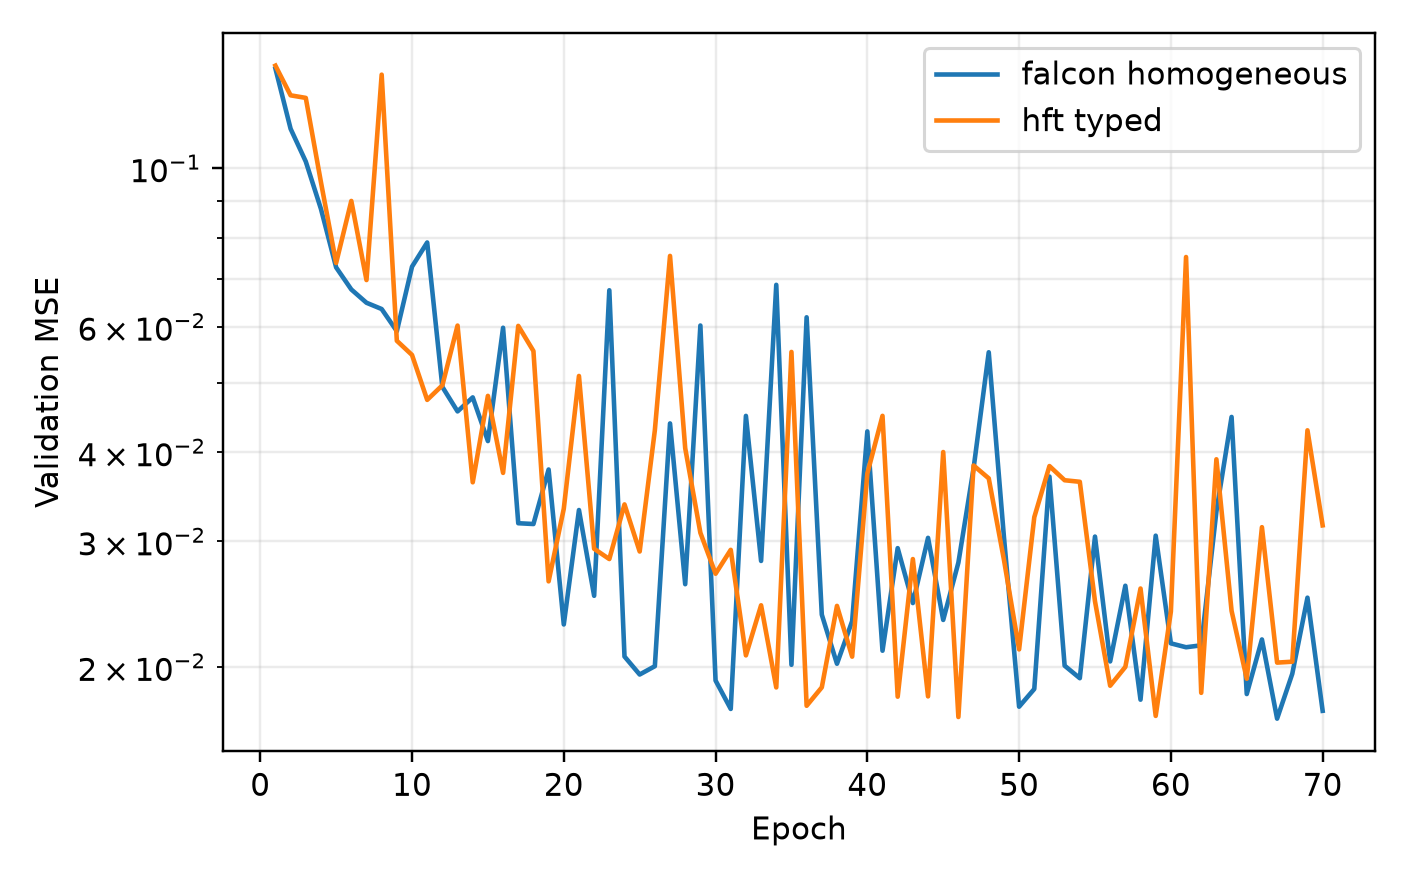
\includegraphics[width=.78\linewidth]{experiments/experiment16_falcon_hft_gnn_20260909/results/training_curves.png}
\caption{EXP16 训练曲线。关注训练/验证是否共同下降、是否出现明显分叉，而不是只看最后一个训练 loss。}
\end{figure}

EXP16 中 homogeneous GNN 的归一化响应 MAE 为 0.0521，typed GNN 为 0.0538，后者没有胜出。这说明“加边类型”本身不会自动带来收益；数据、目标和消息函数必须让类型信息真正可用。

\begin{figure}[H]
\centering
\begin{minipage}{.48\linewidth}\centering
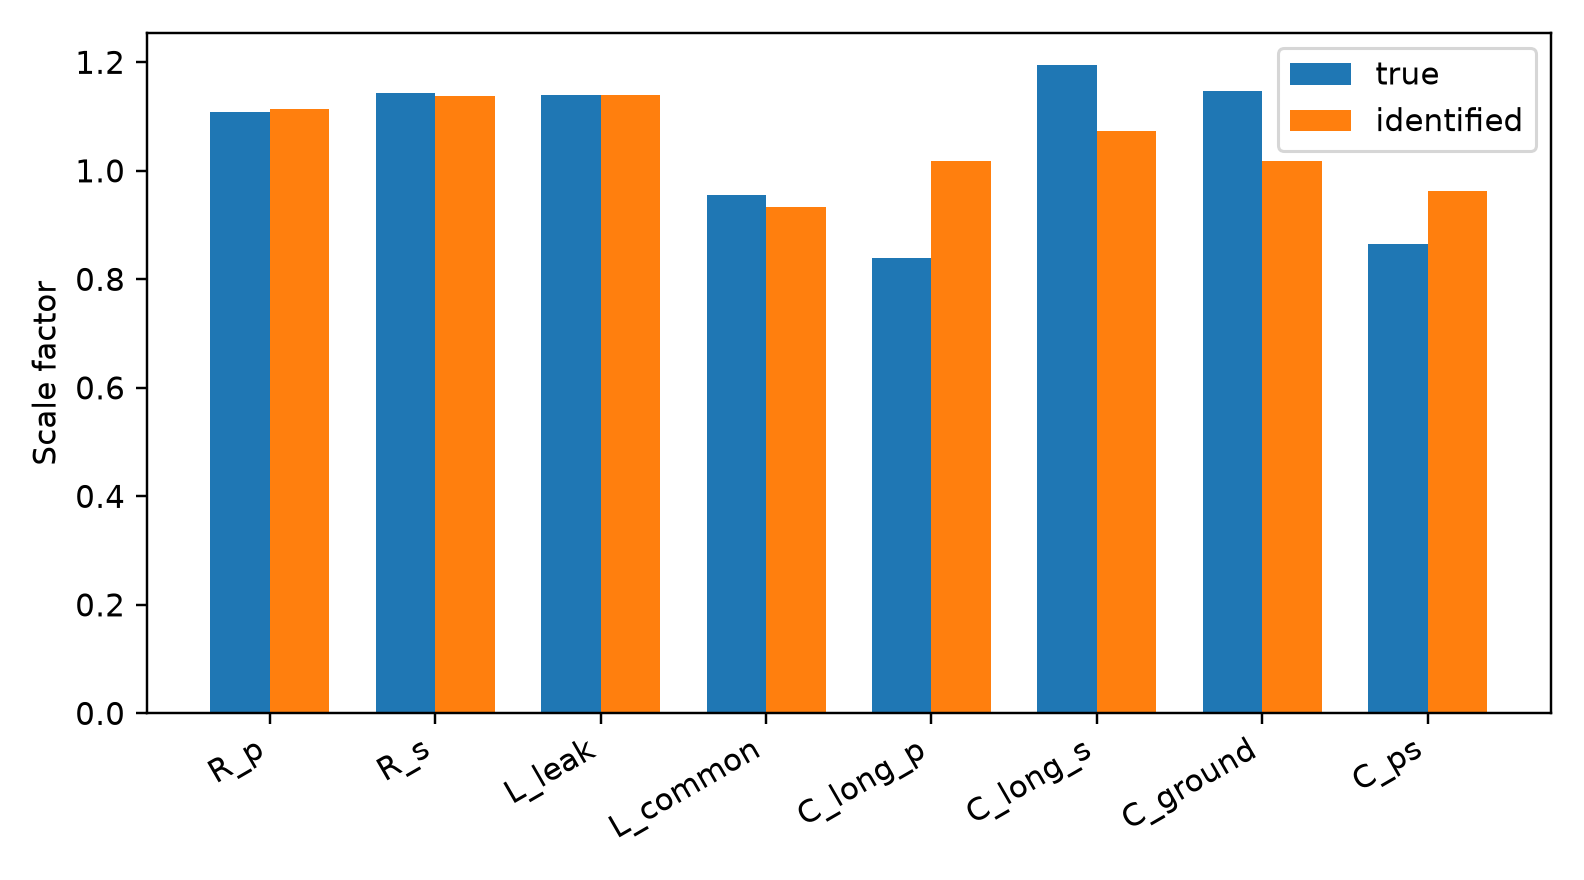
\includegraphics[width=\linewidth]{experiments/experiment16_falcon_hft_gnn_20260909/results/physics_inverse_scales.png}
\caption{物理反演的参数缩放结果。}
\end{minipage}\hfill
\begin{minipage}{.48\linewidth}\centering
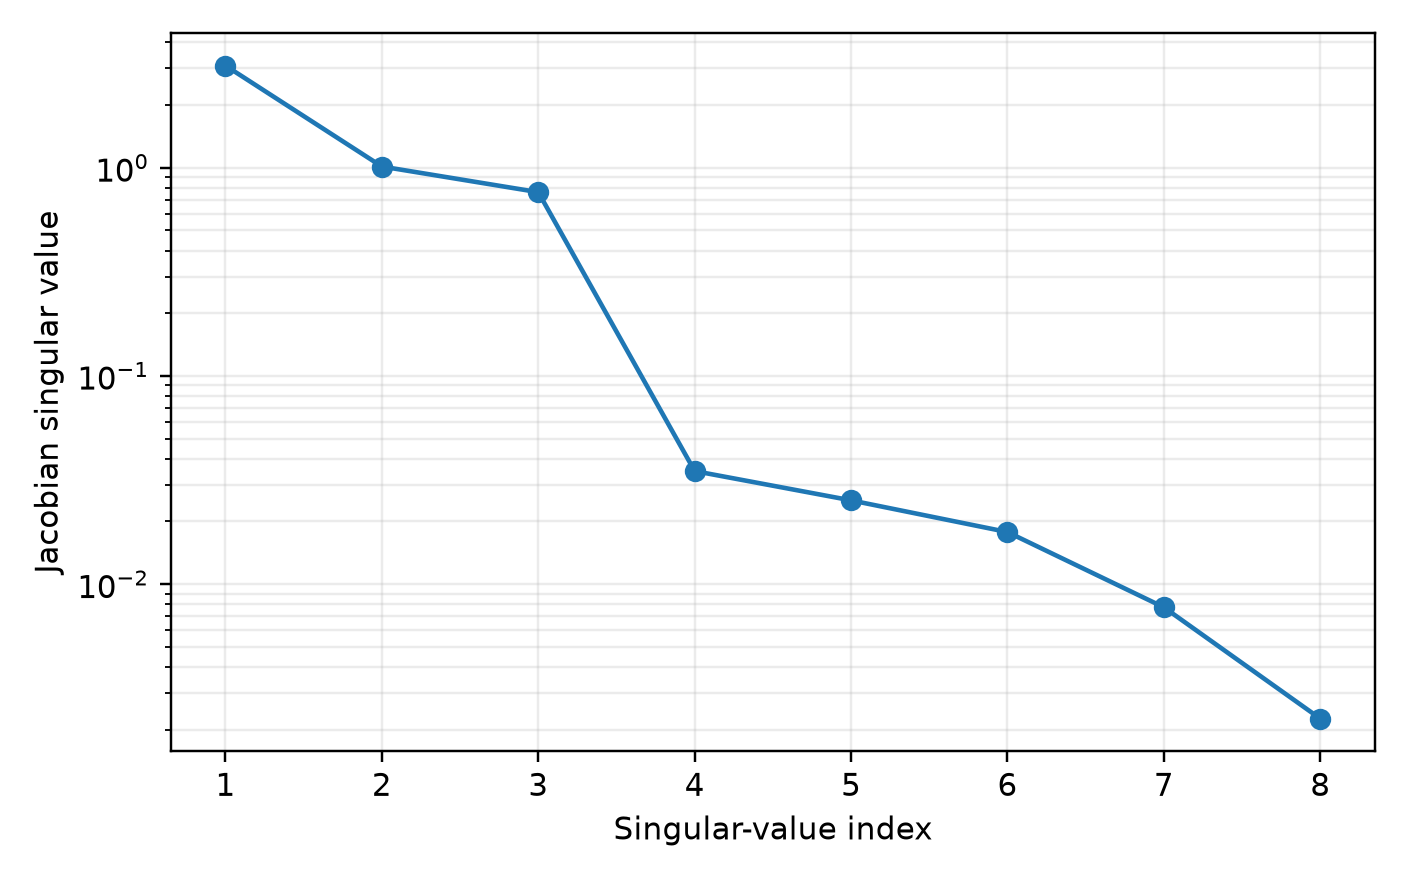
\includegraphics[width=\linewidth]{experiments/experiment16_falcon_hft_gnn_20260909/results/identifiability_spectrum.png}
\caption{灵敏度奇异值谱。}
\end{minipage}
\end{figure}

物理反演响应损失仅 $3.02\times10^{-7}$，但平均参数缩放误差仍为 7.16\%，各电容参数误差约 10\%--21\%。原因是 Jacobian 条件数达到 1368.85：有些参数组合对响应产生近似相同的影响。这是“非唯一/弱可辨识”的直接证据，也是为什么不能让 AI 随意输出完整 $\mat L,\mat C$。

\subsection{EXP17：Fisher/OED 在工程里负责什么}

\begin{figure}[H]
\centering
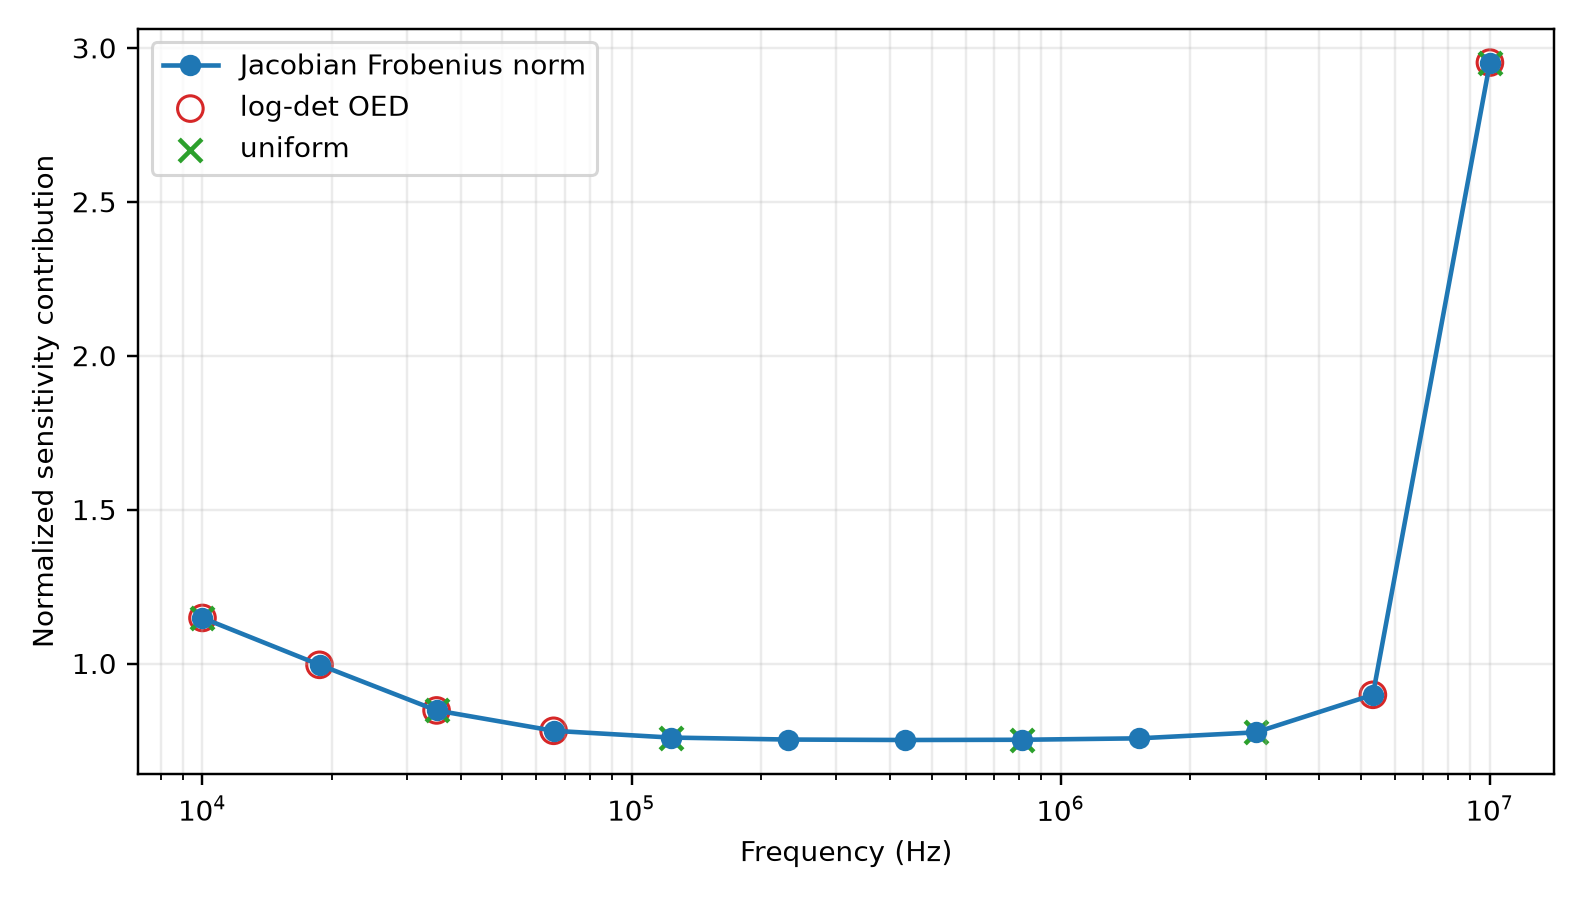
\includegraphics[width=.48\linewidth]{experiments/experiment17_fisher_oed_subspace_20260909/results/frequency_selection.png}\hfill
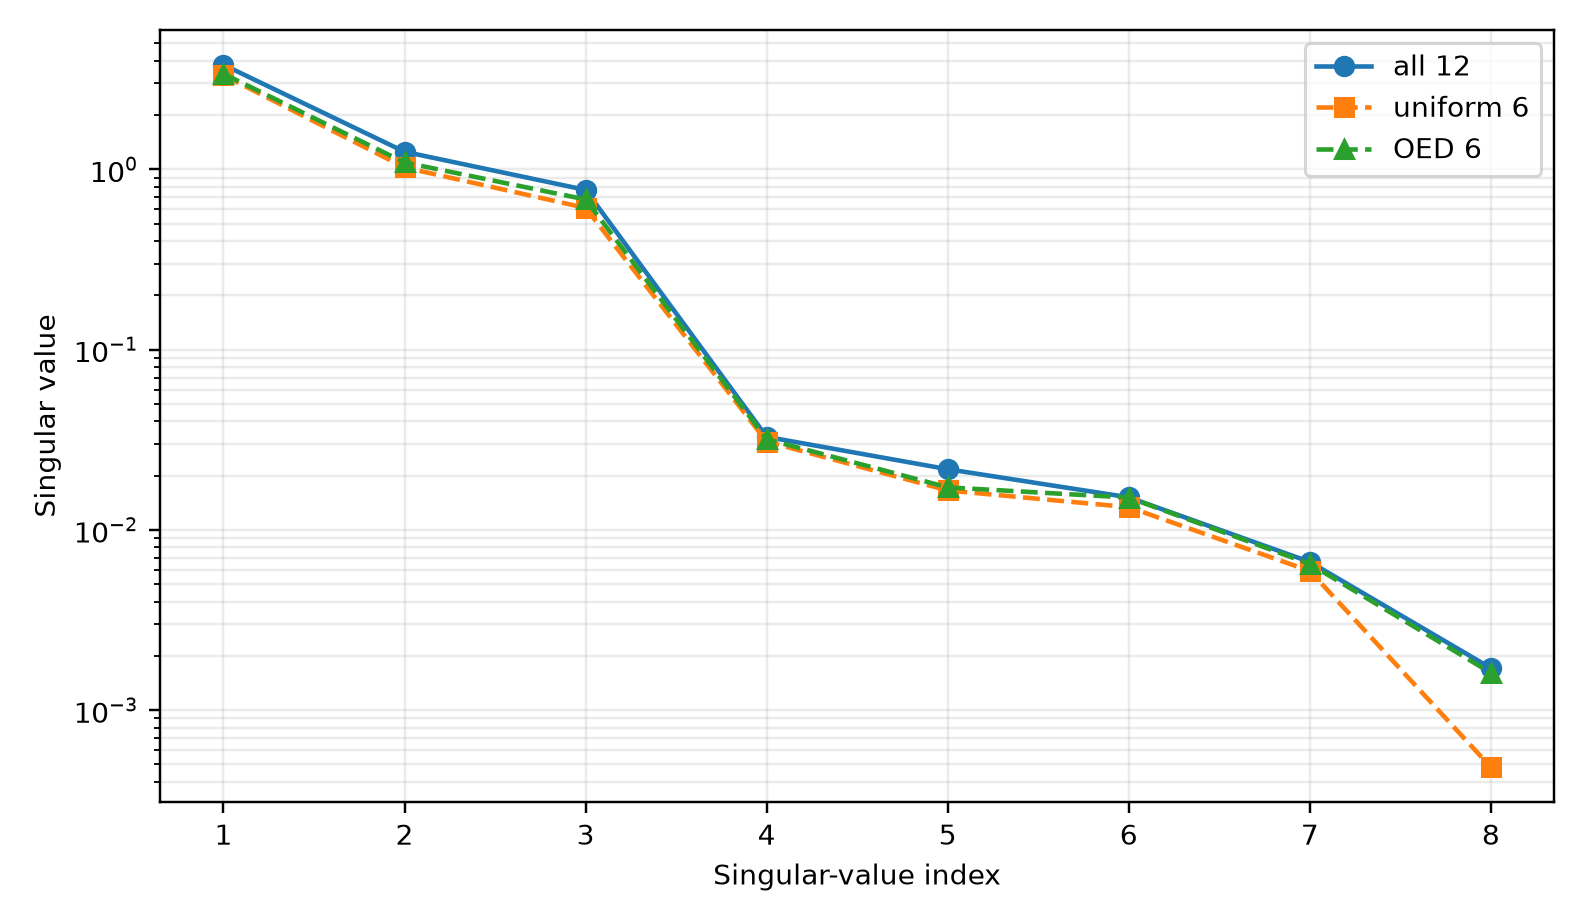
\includegraphics[width=.48\linewidth]{experiments/experiment17_fisher_oed_subspace_20260909/results/fisher_spectrum_comparison.png}
\caption{左：均匀频点与信息驱动频点；右：不同观测设计下 Fisher 特征谱。}
\end{figure}

Fisher 信息矩阵可写为
\begin{equation}
 \mat F=\mat J^{\mathsf H}\mat\Sigma^{-1}\mat J,
 \qquad \mat J=\frac{\partial\mat y}{\partial\bm\theta}.
\end{equation}
它不直接生成预测，而是判断“哪些参数方向能被当前测量区分”。EXP17 的单一 $Y_{11}$、$Y_{22}$ 或 $Y_{12}$ 条件数约达 $10^9$--$10^{10}$，说明只看一个矩阵元素极易退化；全端口和合理选频明显改善数值条件。

\begin{figure}[H]
\centering
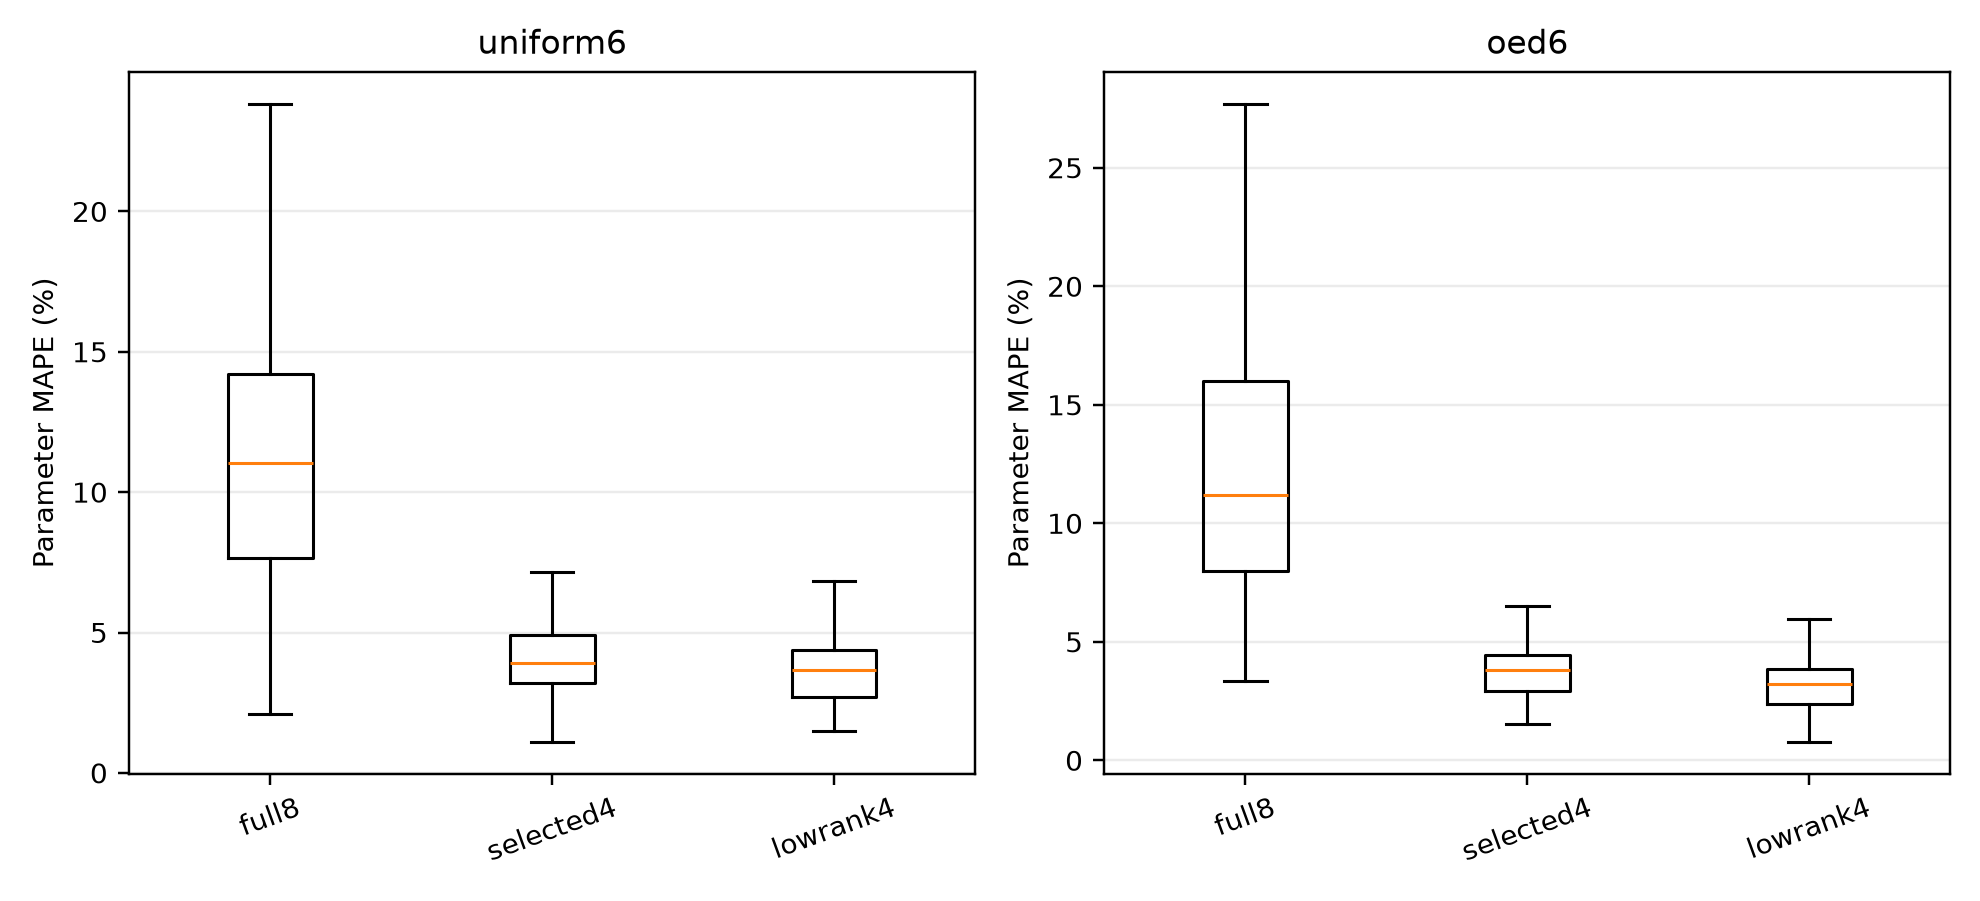
\includegraphics[width=.72\linewidth]{experiments/experiment17_fisher_oed_subspace_20260909/results/monte_carlo_parameter_error.png}
\caption{EXP17 Monte Carlo 参数误差。selected4 和 lowrank4 优于盲目估计 full8。}
\end{figure}

Monte Carlo 中 full8 MAPE 为 12.59\%，Fisher 选出的 selected4 为 3.86\%，低秩 4 维为 3.20\%。结论不是“频率永远可以人为选择”，而是：\key{无论自然 PWM 提供哪些频率，在线算法都应按实际谱能量、噪声和灵敏度对有效信息加权，并限制只更新可辨识子空间。}

\subsection{EXP18：三种 GNN 的真实结论}

\begin{figure}[H]
\centering
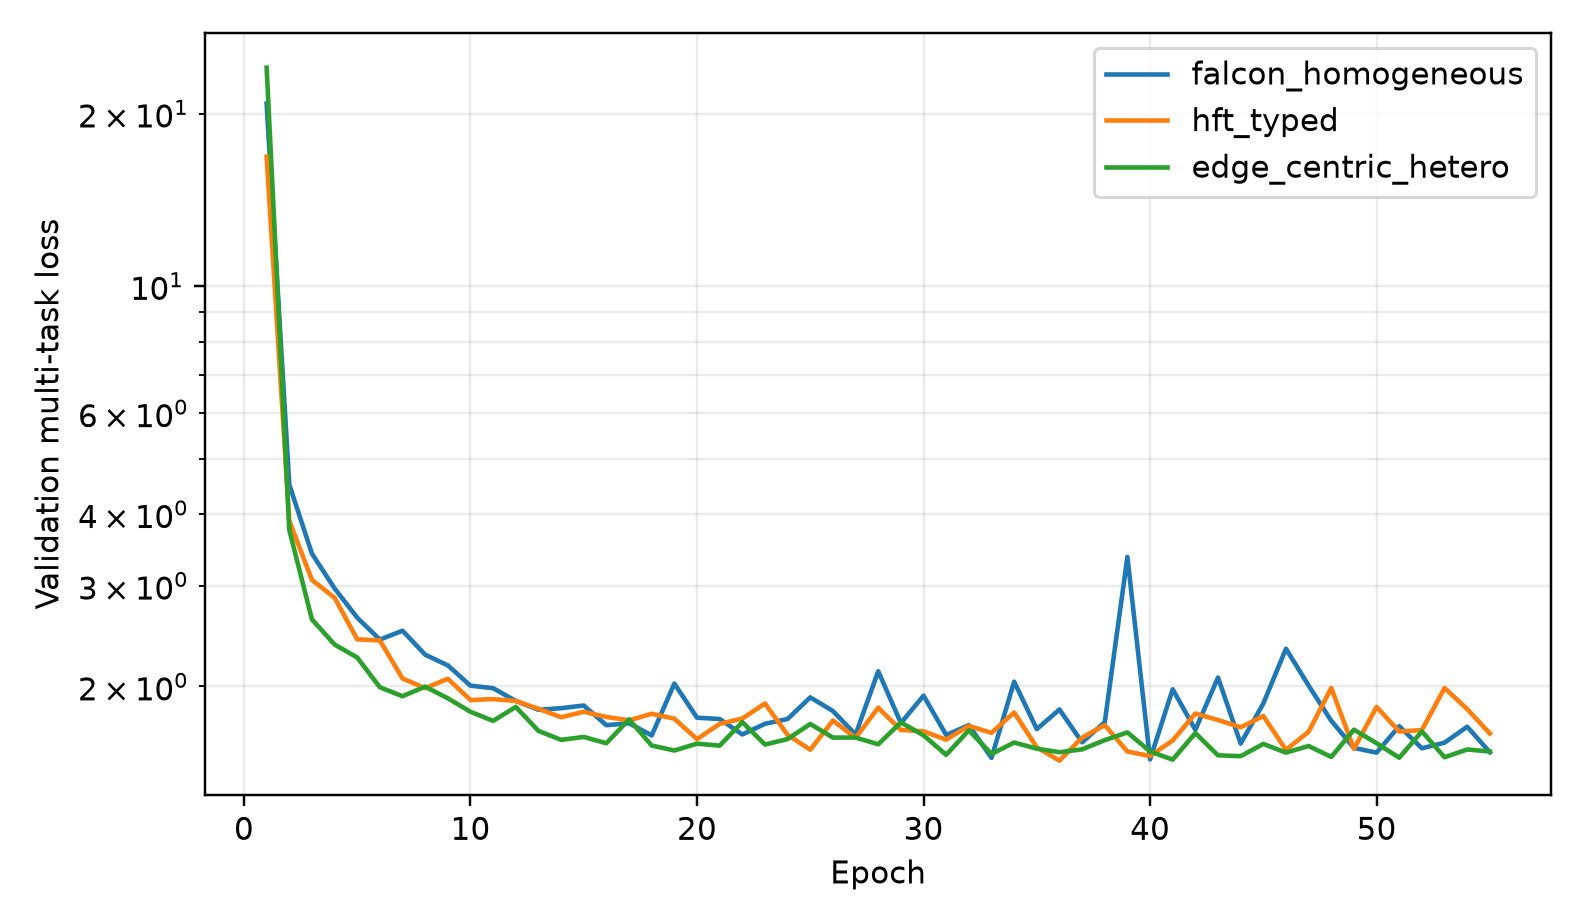
\includegraphics[width=.48\linewidth]{experiments/experiment18_local_hetero_gnn_20260910/results/residual/training_curves.png}\hfill
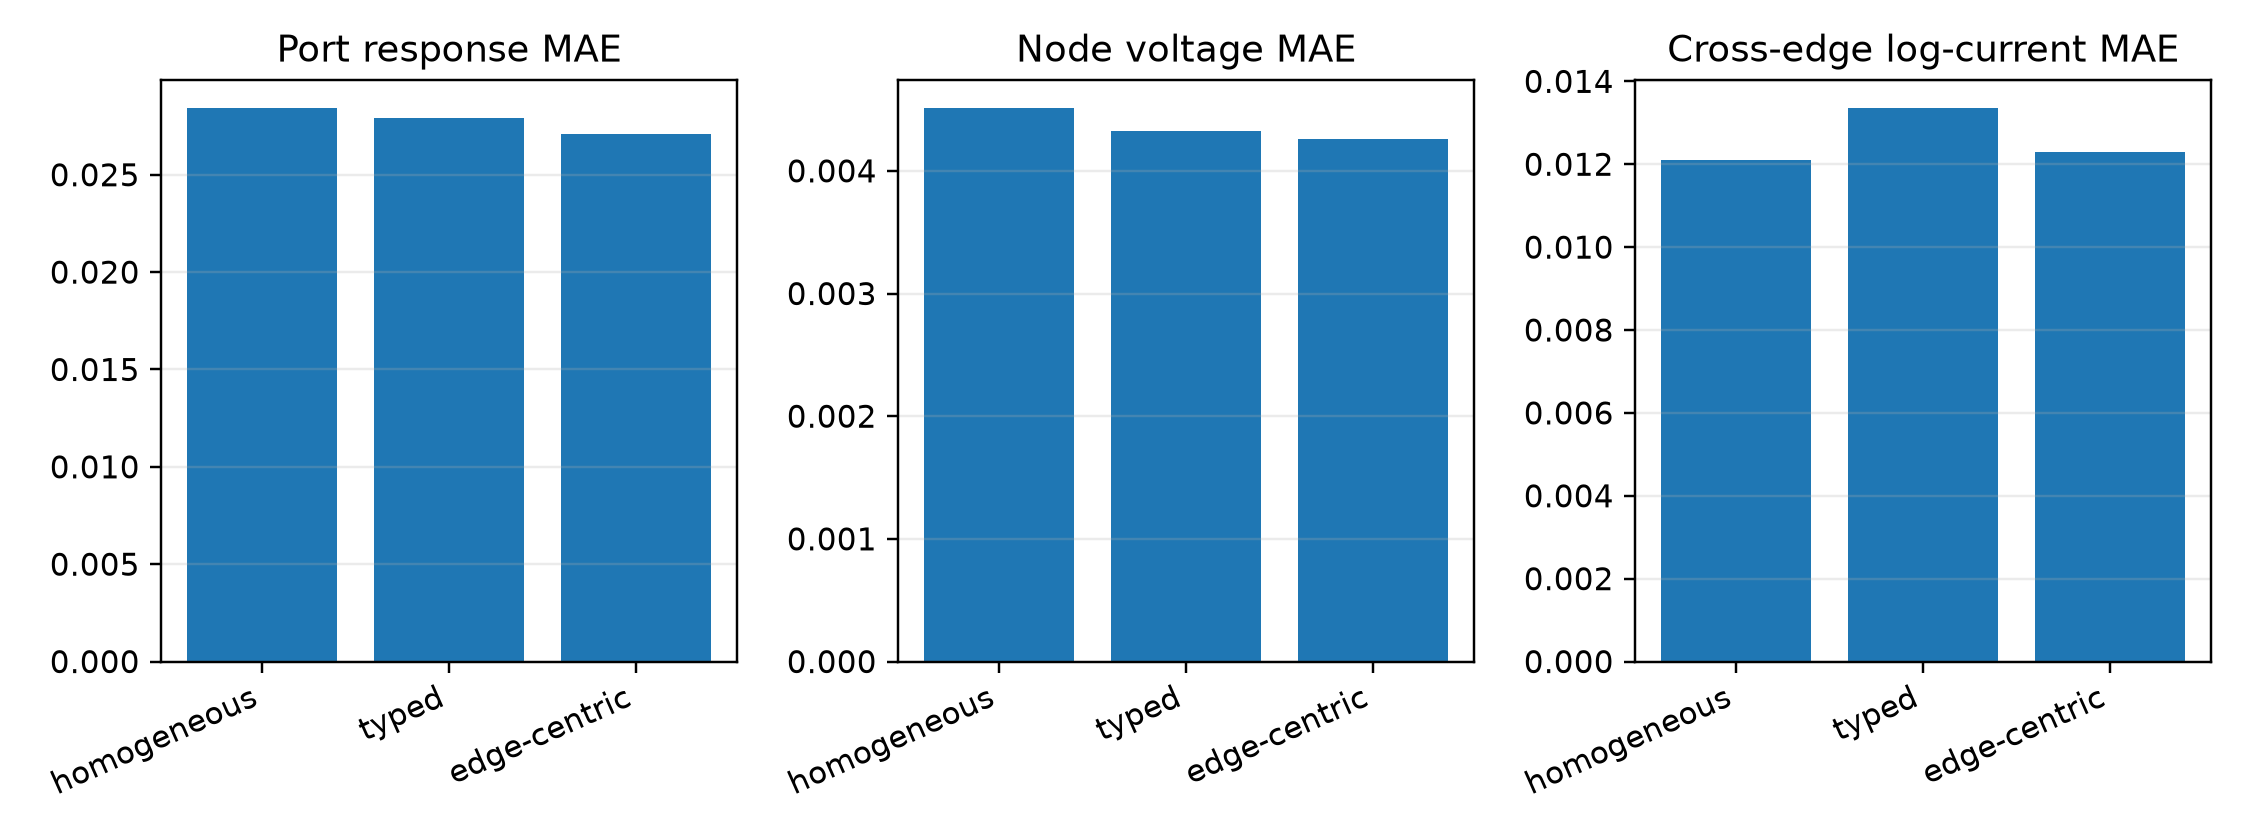
\includegraphics[width=.48\linewidth]{experiments/experiment18_local_hetero_gnn_20260910/results/residual/test_task_comparison.png}
\caption{EXP18 residual 模式训练曲线与测试任务对比。柱子越低越好。}
\end{figure}

\begin{table}[H]
\centering
\caption{EXP18 residual 测试结果}
\begin{tabular}{lcccc}
\toprule
模型 & 端口 MAE & 节点 MAE & 边电流 log MAE & 峰值命中率\\
\midrule
Homogeneous & 0.02845 & 0.004515 & \textbf{0.01211} & 12.08\%\\
Typed & 0.02790 & 0.004328 & 0.01337 & \textbf{13.33\%}\\
Edge-centric & \textbf{0.02707} & \textbf{0.004263} & 0.01230 & 12.50\%\\
\bottomrule
\end{tabular}
\end{table}

Edge-centric 相对 homogeneous 的端口和节点误差改善分别约 4.84\% 和 5.58\%，但边电流反而差约 1.65\%。因此本次结论是“局部残差任务上出现了小幅结构优势”，不是“异构 GNN 已显著优于 FALCON baseline”。

\begin{figure}[H]
\centering
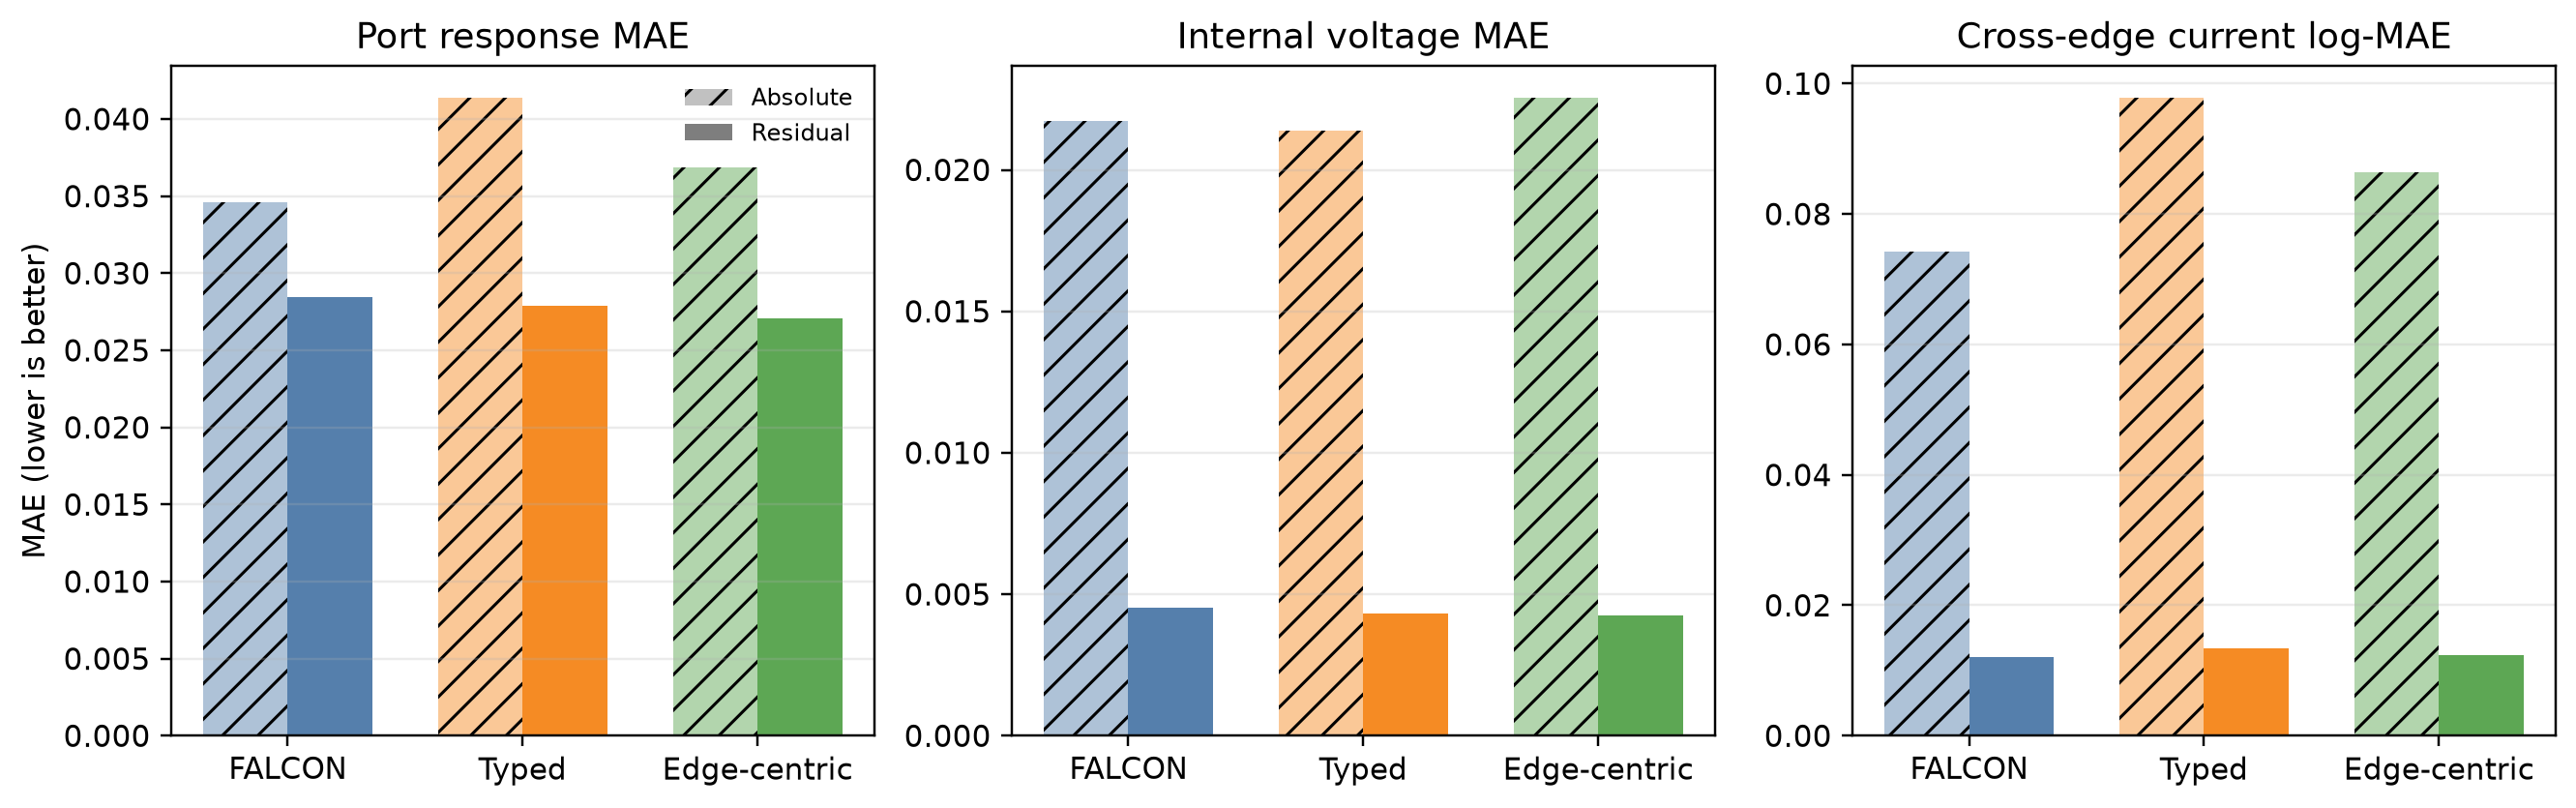
\includegraphics[width=.70\linewidth]{experiments/experiment18_local_hetero_gnn_20260910/results/ablation_absolute_vs_residual.png}
\caption{Absolute 与 residual 学习对比。Residual 把标称物理响应交给教师，只让网络学习偏差，通常更容易。}
\end{figure}

Absolute 模式中 edge-centric 的无源率为 87.33\%，高于 homogeneous 的 76.92\%，说明边物理和无源惩罚有帮助，但距离严格物理保证仍有差距。Absolute 的峰值命中率三者都是 100\%，而 residual 只有 12\%--13\%；前者很可能由固定的绝对峰值结构主导，不能作为真正的局部缺陷定位证据。更严苛的 residual 结果才表明峰值位置尚未解决。

按拓扑看，edge-centric residual 的峰值命中率从 $4+4$ 的 28.75\% 降到 $6+6$ 的 7.5\%、$8+8$ 的 1.25\%。匝数增加后候选位置增多，局部极值间差距变小，精确索引分类迅速变难。后续应增加 top-$k$、位置距离误差和峰值幅值误差，而不是只用 exact hit。

\section{这些结果对整个参数辨识工程有什么作用}

\subsection{已经得到的能力}

\begin{enumerate}
\item 已有可验证的匝级矩阵教师，互易性误差 $1.32\times10^{-14}$、内部 KCL 残差 $5.11\times10^{-11}$、最小实部导纳特征值为正，说明标签生成器数值自洽。
\item 已能在不同匝数和未见 DAB 工况上预测端口、节点、边三类量，证明图数据管线和 CUDA 多任务训练可运行。
\item 已通过 EXP16/17 证明“响应拟合”与“参数唯一恢复”不是一回事，并获得 Fisher 低维化依据。
\end{enumerate}

\subsection{尚未得到的能力}

\begin{enumerate}
\item 网络当前输入中已经含有参数值/残差信息，所以它是参数图到响应的正向映射，\textbf{不是}测量到参数的逆映射。
\item 尚未从 $v_1,i_1,v_2,i_2$ 自动恢复 $C_{ij},M_{ij}$ 或其变化。
\item 尚未使用 COMSOL/实测标签，也没有探头带宽、同步误差、死区、$C_{\rm oss}$ 和真实共模回路。
\item 尚未达到可宣称工程应用的精度；目前可宣称的是“方法链可行、关键瓶颈已识别”。
\end{enumerate}

\subsection{最终在线辨识应怎样接上}

未来不是让网络从四条波形输出成百上千个自由矩阵元素，而是：
\begin{equation}
 \bm z=E_{\rm meas}\!\left(\{V_1,I_1,V_2,I_2\}_{f,w},\bm u_{\rm DAB}\right),
\end{equation}
\begin{align}
 \mat C(\bm z)&=\mat C_0+\sum_{q=1}^{r_C}z_q^{C}\mat B_q^{C},\\
 \mat L(\bm z)&=\mat L_0+\sum_{q=1}^{r_L}z_q^{L}\mat B_q^{L},
\end{align}
其中 $\mat B_q$ 是由 FEM、图结构或 Fisher/SVD 得到的物理变化基。随后用精确矩阵解码器重构测量：
\begin{equation}
 \hat{\mat I}_{f,w}=\mat Y_{\rm port}(f;\mat R,\mat L(\bm z),\mat C(\bm z))\mat V_{f,w}.
\end{equation}
训练/在线优化目标应包含
\begin{equation}
 \mathcal L_{\rm online}=\mathcal L_{VI}+\lambda_{\rm prior}\|\bm z\|^2
 +\lambda_{\rm Fisher}\bm z^{\mathsf T}(\mat F+\epsilon\mat I)^{-1}\bm z
 +\mathcal L_{\rm passive}+\mathcal L_{\rm reciprocal}.
\end{equation}
这样 AI 提供非线性测量编码和跨工况先验，物理矩阵保证输出可解释，Fisher 限制网络只沿可观测方向修改参数。

\section{如何复现实验以及每一步看什么}

在仓库工作树 \code{D:/高频变压器/hft-worktrees/experiments} 下，先加载项目配置的 Python/CUDA 环境，再运行各实验目录中的入口脚本。具体文件名以各目录 README 为准。推荐检查顺序如下：
\begin{enumerate}
\item 运行 EXP16：先确认 GNN 训练可复现，再观察低响应损失与参数误差并存；
\item 运行 EXP17：检查 Fisher 谱、选频和 Monte Carlo，理解为何必须降到可辨识子空间；
\item 运行 EXP18 absolute：检查端口精度和无源率；
\item 运行 EXP18 residual：检查局部变化学习和跨拓扑定位；
\item 查看每个 \code{metrics.json}，不要只凭柱状图判断；确认随机种子、数据划分、CUDA 设备和模型权重均已保存。
\end{enumerate}

阅读训练曲线时，若训练损失下降而验证损失上升，是过拟合；二者都高是容量、输入或标签问题；二者共同下降并稳定才说明优化收敛。比较模型时必须保证使用同一数据划分、同一输出头、相近参数量和相同训练预算。

\section{下一步最合理的实验}

\key{下一步不应继续堆更复杂 GNN 名称，而应把“正向代理”接成一个最小在线反演闭环。}

建议 EXP19 分两阶段：
\begin{enumerate}
\item \textbf{可辨识低维图参数：}由 EXP17 Fisher/SVD 为 $\mat C,\mat L$ 构造 4--8 个变化基，只让待估变量为 $\bm z$；先用精确矩阵教师生成带噪 DAB 多窗口数据。
\item \textbf{测量编码器：}输入多窗口 $V_1,I_1,V_2,I_2$ 复频谱及工况，输出 $\hat{\bm z}$；通过精确矩阵层重构电流，并与物理最小二乘、MLP、FALCON-style homogeneous encoder 和异构 encoder 比较。
\end{enumerate}

验收指标至少包括：参数子空间误差、端口重构误差、未见工况泛化、噪声鲁棒性、无源/互易率、推理时间、置信区间覆盖率；局部定位增加 top-3 命中率和匝位距离误差。等这一闭环稳定后，再用 COMSOL 产生少量独立教师数据，并用仿真预训练加少量实测微调。

\section{一句话结论}

目前实验已证明：\key{匝级全耦合矩阵可以被组织成 HFT 专用异构图，GNN 能在一定程度上学习端口--内部--边的联合响应；但参数反演受可辨识性支配，真正在线化必须是“测量编码器 $+$ 低维图参数 $+$ 精确物理解码器 $+$ Fisher 约束”，而不是从少量端口数据自由猜测整个矩阵。}

\appendix
\section{关键结果速查}
\begin{longtable}{p{0.12\linewidth}p{0.32\linewidth}p{0.47\linewidth}}
\toprule
实验 & 关键数字 & 应得结论\\
\midrule
EXP16 & GNN MAE 0.0521/0.0538；条件数 1368.85；参数平均缩放误差 7.16\% & 图 baseline 可跑，但响应拟合不保证参数唯一\\
EXP17 & full8 12.59\%，selected4 3.86\%，lowrank4 3.20\% & Fisher/OED 的价值是选择可辨识方向，不只是选一个“最佳频率”\\
EXP18 & residual edge-centric 端口 0.02707、节点 0.004263、边电流 0.01230；峰值 12.5\% & 异构边有小幅正向价值，局部定位和严格物理性仍需加强\\
\bottomrule
\end{longtable}

\section{术语速查}
\begin{description}
\item[Forward surrogate] 已知图结构和参数，快速预测响应。
\item[Inverse identification] 已知测量响应，估计未知参数；可能非唯一。
\item[Residual learning] 物理模型给标称结果，网络只学剩余误差。
\item[Fisher information] 衡量测量对参数变化的可分辨程度。
\item[Kron reduction] 消去内部节点，得到等效端口导纳，同时可恢复内部状态。
\item[Passivity] 网络不凭空产生能量；频域常检查 $\Re\{\mat Y\}\succeq0$。
\item[Reciprocity] 无源互易网络通常满足 $\mat Y=\mat Y^{\mathsf T}$。
\end{description}

\end{document}
